%% abtex2-modelo-trabalho-academico.tex, v<VERSION> laurocesar
%% Copyright 2012-<COPYRIGHT_YEAR> by abnTeX2 group at http://www.abntex.net.br/ 
%%
%% This work may be distributed and/or modified under the
%% conditions of the LaTeX Project Public License, either version 1.3
%% of this license or (at your option) any later version.
%% The latest version of this license is in
%%   http://www.latex-project.org/lppl.txt
%% and version 1.3 or later is part of all distributions of LaTeX
%% version 2005/12/01 or later.
%%
%% This work has the LPPL maintenance status `maintained'.
%% 
%% The Current Maintainer of this work is the abnTeX2 team, led
%% by Lauro César Araujo. Further information are available on 
%% http://www.abntex.net.br/
%%
%% This work consists of the files abntex2-modelo-trabalho-academico.tex,
%% abntex2-modelo-include-comandos and abntex2-modelo-references.bib
%%

% ------------------------------------------------------------------------
% ------------------------------------------------------------------------
% abnTeX2: Modelo de Trabalho Academico (tese de doutorado, dissertacao de
% mestrado e trabalhos monograficos em geral) em conformidade com 
% ABNT NBR 14724:2011: Informacao e documentacao - Trabalhos academicos -
% Apresentacao
% ------------------------------------------------------------------------
% ------------------------------------------------------------------------

\documentclass[
	% -- opções da classe memoir --
	12pt,				% tamanho da fonte
	openright,			% capítulos começam em pág ímpar (insere página vazia caso preciso)
	twoside,			% para impressão em recto e verso. Oposto a oneside
	a4paper,			% tamanho do papel. 
	% -- opções da classe abntex2 --
	%chapter=TITLE,		% títulos de capítulos convertidos em letras maiúsculas
	%section=TITLE,		% títulos de seções convertidos em letras maiúsculas
	%subsection=TITLE,	% títulos de subseções convertidos em letras maiúsculas
	%subsubsection=TITLE,% títulos de subsubseções convertidos em letras maiúsculas
	% -- opções do pacote babel --
	english,			% idioma adicional para hifenização
	french,				% idioma adicional para hifenização
	spanish,			% idioma adicional para hifenização
	brazil				% o último idioma é o principal do documento
	]{abntex2}

% ---
% Pacotes básicos 
% ---
\usepackage{lmodern}			% Usa a fonte Latin Modern			
\usepackage[T1]{fontenc}		% Selecao de codigos de fonte.
\usepackage[utf8]{inputenc}		% Codificacao do documento (conversão automática dos acentos)
\usepackage{indentfirst}		% Indenta o primeiro parágrafo de cada seção.
\usepackage{color}				% Controle das cores
\usepackage{graphicx}			% Inclusão de gráficos
\usepackage{microtype} 			% para melhorias de justificação
\usepackage{enumerate}			% para numeração das listas 
\usepackage{enumitem}			% para numeração das listas 
\setlist[enumerate]{label*=\arabic*.}
% ---


% ---
% Pacotes de citações
% ---
\usepackage[brazilian,hyperpageref]{backref}	 % Paginas com as citações na bibl
\usepackage[alf]{abntex2cite}	% Citações padrão ABNT

% --- 
% CONFIGURAÇÕES DE PACOTES
% --- 


% ---
% Configurações do pacote backref
% Usado sem a opção hyperpageref de backref
\renewcommand{\backrefpagesname}{Citado na(s) página(s):~}
% Texto padrão antes do número das páginas
\renewcommand{\backref}{}
% Define os textos da citação
\renewcommand*{\backrefalt}[4]{
	\ifcase #1 %
		Nenhuma citação no texto.%
	\or
		Citado na página #2.%
	\else
		Citado #1 vezes nas páginas #2.%
	\fi}%
% ---

% ---
% Informações de dados para CAPA e FOLHA DE ROSTO
% ---
\titulo{Análise e classificação de comentários}
\autor{Fabrício Velôso de Jesus}
\local{Brasil}
\data{2018, v1.0}
\orientador{Tiago Palma Pagano}

\instituicao{%
  Universidade Federal do Recôncavo da Bahia - UFRB
  Bacharelado em Ciências Exatas e Tecnológicas}
\tipotrabalho{Monografia (Graduação)}
% O preambulo deve conter o tipo do trabalho, o objetivo, 
% o nome da instituição e a área de concentração 
\preambulo{Trabalho monografico apresentado para obtenção do grau de bacharel em ciências exatas e tecnológicas.}
% ---


% ---
% Configurações de aparência do PDF final

% alterando o aspecto da cor azul
\definecolor{blue}{RGB}{41,5,195}

% informações do PDF
\makeatletter
\hypersetup{
     	%pagebackref=true,
		pdftitle={\@title}, 
		pdfauthor={\@author},
    	pdfsubject={\imprimirpreambulo},
	    pdfcreator={LaTeX with abnTeX2},
		pdfkeywords={abnt}{latex}{abntex}{abntex2}{trabalho acadêmico}, 
		colorlinks=true,       		% false: boxed links; true: colored links
    	linkcolor=blue,          	% color of internal links
    	citecolor=blue,        		% color of links to bibliography
    	filecolor=magenta,      		% color of file links
		urlcolor=blue,
		bookmarksdepth=4
}
\makeatother
% --- 

% ---
% Posiciona figuras e tabelas no topo da página quando adicionadas sozinhas
% em um página em branco. Ver https://github.com/abntex/abntex2/issues/170
\makeatletter
\setlength{\@fptop}{5pt} % Set distance from top of page to first float
\makeatother
% ---

% ---
% Possibilita criação de Quadros e Lista de quadros.
% Ver https://github.com/abntex/abntex2/issues/176
%
\newcommand{\quadroname}{Quadro}
\newcommand{\listofquadrosname}{Lista de quadros}

\newfloat[chapter]{quadro}{loq}{\quadroname}
\newlistof{listofquadros}{loq}{\listofquadrosname}
\newlistentry{quadro}{loq}{0}

% configurações para atender às regras da ABNT
\setfloatadjustment{quadro}{\centering}
\counterwithout{quadro}{chapter}
\renewcommand{\cftquadroname}{\quadroname\space} 
\renewcommand*{\cftquadroaftersnum}{\hfill--\hfill}

\setfloatlocations{quadro}{hbtp} % Ver https://github.com/abntex/abntex2/issues/176
% ---

% --- 
% Espaçamentos entre linhas e parágrafos 
% --- 

% O tamanho do parágrafo é dado por:
\setlength{\parindent}{1.3cm}

% Controle do espaçamento entre um parágrafo e outro:
\setlength{\parskip}{0.2cm}  % tente também \onelineskip

% ---
% compila o indice
% ---
\makeindex
% ---

% ----
% Início do documento
% ----
\begin{document}

% Seleciona o idioma do documento (conforme pacotes do babel)
%\selectlanguage{english}
\selectlanguage{brazil}

% Retira espaço extra obsoleto entre as frases.
\frenchspacing 

% ----------------------------------------------------------
% ELEMENTOS PRÉ-TEXTUAIS
% ----------------------------------------------------------
% \pretextual

% ---
% Capa
% ---
\imprimircapa
% ---

% ---
% Folha de rosto
% (o * indica que haverá a ficha bibliográfica)
% ---
\imprimirfolhaderosto*
% ---

% ---
% Inserir a ficha bibliografica
% ---

% Isto é um exemplo de Ficha Catalográfica, ou ``Dados internacionais de
% catalogação-na-publicação''. Você pode utilizar este modelo como referência. 
% Porém, provavelmente a biblioteca da sua universidade lhe fornecerá um PDF
% com a ficha catalográfica definitiva após a defesa do trabalho. Quando estiver
% com o documento, salve-o como PDF no diretório do seu projeto e substitua todo
% o conteúdo de implementação deste arquivo pelo comando abaixo:
%
% \begin{fichacatalografica}
%     \includepdf{fig_ficha_catalografica.pdf}
% \end{fichacatalografica}

% ---

% ---
% RESUMOS
% ---

% resumo em português
\setlength{\absparsep}{18pt} % ajusta o espaçamento dos parágrafos do resumo
\begin{resumo}
 

 \textbf{Palavras-chave}: 
\end{resumo}

% resumo em inglês
\begin{resumo}[Abstract]
 \begin{otherlanguage*}{english}
   

   \vspace{\onelineskip}
 
   \noindent 
   \textbf{Keywords}: 
 \end{otherlanguage*}
\end{resumo}


% ---
% inserir lista de ilustrações
% ---
\pdfbookmark[0]{\listfigurename}{lof}
\listoffigures*
\cleardoublepage
% ---

% ---
% inserir lista de quadros
% ---
\pdfbookmark[0]{\listofquadrosname}{loq}
\listofquadros*
\cleardoublepage
% ---

% ---
% inserir lista de tabelas
% ---
\pdfbookmark[0]{\listtablename}{lot}
\listoftables*

\cleardoublepage
% ---

% ---
% inserir lista de abreviaturas e siglas
% ---
\begin{siglas}
  \item[BMU] \emph{Best Match Unit}  	
  \item[IA] Sigla para Inteligência Artificial
  \item[KDD] \emph{Knowledge Discovery in Database}, em portugês Descoberta de Conhecimento em Bases de Dados
  \item[SOM] \emph{Self-Organizing Map}, em portugês Mapas auto organizáveis
  \item[RNAs] Sigla para Redes Neurais Artificiais
  
  
\end{siglas}
% ---

% ---
% inserir lista de símbolos
% ---
\begin{simbolos}
  \item[$ \Gamma $] Letra grega Gama
  
\end{simbolos}
% ---

% ---
% inserir o sumario
% ---
\pdfbookmark[0]{\contentsname}{toc}
\tableofcontents*
\cleardoublepage
% ---



% ----------------------------------------------------------
% ELEMENTOS TEXTUAIS
% ----------------------------------------------------------
\textual

% ----------------------------------------------------------
% Introdução (exemplo de capítulo sem numeração, mas presente no Sumário)
% ----------------------------------------------------------
\chapter{Introdução}
% ----------------------------------------------------------

\section{Objetivo}
Analisar e classificar comentários de twitter segundo seu caráter misógino.
\section{Objetivos específicos}
Utilizar métodos capazes de classificar os comentários segundo seu caráter misógino.
Dentro deste comportamento de aversão às mulheres existem subcategorias, que devem ser declaradas e evidenciadas na classificação.

Analisar caracteristicas comuns as frases que pertecem ao mesmo grupo e determinar a ocorrência e relevância de determinadas palavras para a identificação.

Determinar se tal comportamento possui direcionamento a um usuário em específico, ou é realizado de forma a generalizar todas as mulheres.

\section{Justificativa}
Como consequência, a análise dos resultados obtidos neste trabalho poderá prover um padrão especifico referente ao comportamento de usuários misóginos no twitter.

\section{Metodologia}
Aplicar métodos de mineração de dados em textos para realizar o ajuste dos dados existentes na base. 

Utilizar aprendizado de máquina nos dados ajustados para criar uma rotina de classificação das frases.
A proposta aqui é com o auxílio de redes neurais, evidenciar dados específicos encontrados em comentários que refletem um cunho misógino, no qual destacamos o método de mapas auto organizáveis com o intuito de evidenciar características comuns em frases que possuem a mesma classificação.


\section{Problematização}
Com auxílio de métodos inerentes a inteligência artificial é possível determinar a existência de misoginia em um comentário?

Através do agrupamento de características é praticável a classificação das frases misóginas em subcategorias?

Existe um padrão para comentários que apresentam cunho misógino? 
% Capitulo de revisão de literatura
% ---
\chapter{Referêncial Teórico}
Neste capítulo as referências conceituais e  conceitos envolvidos neste trabalho serão descritos. Partindo da definição de misoginia, passando pelas técnicas envolvidas, e arrematando com as concepções de analise dos dados.

\section{Misoginia}
Segundo \citeonline{bloch1995misoginia} qualquer definição essencialista da mulher, seja ela negativa ou positiva, feita por um homem ou uma mulher, é a definição fundamental de misoginia. \citeonline{liviadeodato2017} também define misoginia como o termo utilizado para caracterizar a antipatia, o desprezo ou a aversão as mulheres.

O constante conflito de ideologias entre gerações mostra como o preconceito surge, tendo em vista as mudanças em âmbitos sociais e em relações de convivência, econômicas, pessoais, entre outras, ao passar dos anos, além da dificuldade de adaptação de costumes e pensamentos. A misoginia, base de vários outros preconceitos é a mais alarmante e evidente entre as discriminações que assolam o Brasil. \cite{da2017valores}

Conforme \citeonline{pazo2016misoginia} e \citeonline{alvares2017pos} a misoginia em redes sociais é um comportamento brutal e insultuoso, que vão desde feedback negativo à aparência a ameaças mais sérias. Onde os perseguidores se valem da principal característica da navegação, o anonimato, para disseminarem  seus ataques.

A misoginia pode se manifestar de diferentes maneiras e manifestações ofensivas às mulheres e não é raro de se encontrar em diversos ambientes virtuais. Não apenas nas mais utilizadas redes sociais virtuais, como também em páginas voltadas para discussões anônimas.\cite{pazo2016misoginia}


\subsection{Classificação de comportamento misógino}
O comportamento misógino em um tweet deve ser classificado como pertencente a uma das seguintes categorias, conforme descrito por \cite{fersini2018overview}:
	\begin{itemize}
	\item \emph{Stereotype \& Objectitication} (Estereótipo \& Objetificação): uma idéia ou imagem de mulher amplamente difundida, porém fixa e simplista; descrição do físico feminino, apelo e/ou comparações a padrões delimitados;
	\item \emph{Dominance} (Domínio): afirmar a superioridade de homens sobre as mulheres para destacar a desigualdade de gênero;
	\item \emph{Derailing}: justificar o abuso de mulheres, rejeitando a responsabilidade masculina; uma tentativa de interronper a conversa, a fim de redirecionar as conversas das mulheres em algo mais confortável para os homens; 
	\item \emph{Sexual Harassment \& Threats of Violence}(Assédio sexual \& Ameaças de violência): descrever ações como avanços sexuais, pedidos de favores sexuais, assédio de natureza sexual; intenção de afirmar fisicamente poder sobre as mulhers através de ameaças de violência;
	\item \emph{Discredit} (Discrédito): insultar as mulheres sem nenhuma intenção maior. 
	\end{itemize}
\section{Mineração de Dados}
Conforme \citeonline{amorim2006conceitos} e  \citeonline{santos2008computaccao} a definição de mineração de dados (\emph{Data Mining}) pode ser descrita como o conjunto de técnicas que permite a extração de conhecimentos, padrões e relações de grandes massas de dados que não seriam descobertas com facilidade a olho nu pelo homem.

A descoberta de padrões constitui-se de um processo que se inicia pela escolha dos dados que documentam de alguma maneira a pergunta que o especialista deseja responder. Os dados são integrados e pré-processados para que sejam entregues estruturados, higienizados, selecionados e padronizados à tarefa de mineração de dados. Na tarefa de mineração aplica-se alguma técnica inteligente capaz de encontrar soluções que auxiliam o especialista na descoberta de uma resposta. O resultado desta tarefa deve ser pós-processado para que se apresentem análises qualitativas e/ou quantitativa dos elementos encontrados e, quando possível, apresentados de maneira que possa ser interpretado de maneira a facilitar a tomada de decisão. \cite[p.569 - p.570]{inproceedings}

Todo este processo citado acima, pode ser chamado de Descoberta de Conhecimento em Base de Dados ou simplismente KDD, consoante \apudonline{fayyad1996kdd}{inproceedings}.

Uma das definições mais utilizadas para o termo KDD é a de Fayyad, que o define como "um processo não trivial de identificação de novos padrões válidos, úteis e compreensíveis".\cite[p.3]{camilo2009mineraccao}

Ainda segundo \citeonline{camilo2009mineraccao}, até agora não é consenso a definição dos termos \emph{Data Mining} e \emph{KDD}. No entanto, todos concordam que o processo de mineração deve ser interativo, iterativo e particionado em fases, comforme visto na \autoref{fig_processo_descoberta}. 

\begin{figure}[htb]
	\caption{\label{fig_processo_descoberta}Processo de Descoberta de Conhecimento em Base de Dados}
	\begin{center}
	    \includegraphics[scale=0.4]{imagens/Processo_de_descoberta_de_conhecimento_em_base_de_dados.pdf}
	\end{center}
	\legend{Fonte: \citeonline[p.570]{inproceedings}}
\end{figure}

\subsection{Tipos de estrutura de dados}
Segundo \citeonline{sargiani2018identificaccao} a estrutura com a qual os dados são apresentados é importante, ela induz de forma direta nas ferramentas que serão utilizadas e nas técnicas de tratamento. Na análise de dados  não estruturados ferramentas que permitem extração de conhecimento a partir de dados sem estrutura são utilizadas. Para dados semi-estruturados as técnicas são definidas  com base no caso em específico. E para dados estruturados bancos relacionais são utilizados.

De acordo com \citeonline{morais2007mineraccao} e \citeonline{sargiani2018identificaccao}, o processo de descoberta de conhecimento em \textbf{dados estruturados} é feito através do uso de ferramentas baseadas em métodos estatísticos, métodos provenientes da área de recuperação de informações e  ontologias, estes dados possuem um formato definido através de algum critério. A informação pode ser representada em \emph{datasets}, tabelas, arquivos multimídia ou arquivos texto. 

Os \textbf{dados semi-estruturados} não possuem um formato adequado para o uso de apenas uma ontologia, porém podem ser identificados, pois possuem algum grau de regularidade.\apud{barros2008hidden}{sargiani2018identificaccao}

Conforme \citeonline{inbook} e \citeonline{sargiani2018identificaccao} os chamados \textbf{dados não estruturados} ocorrem quando a informação não possui nenhum formato reconhecível, comumente correlacionado a linguagem natural, o Twitter, e-mails e conteúdo em fóruns são alguns exemplos, as informações não estão dispostas em tabelas númericas organizadas em linhas e colunas e não possuem um formato adequado para o uso de uma ontologia. A mineração de textos é uma técnica usada pelos sistemas inteligentes que engloba o processamento de dados não estruturados do tipo texto, em outras palavras as \emph{strings} ou sequência de caracteres de um texto.

\section{Mineração de Textos}
A mineração de textos consiste em extrair regularidades , padrões ou tendências para determinados objetivos, essa obtenção de informação é feita em grandes volumes de textos em linguagem natural. É um campo novo e multidisciplinar que inclui conhecimento de áreas como Estatística, Informática, Linguistica e Ciência Cognitiva. \citeonline{aranha2006tecnologia}

Conforme \citeonline{sargiani2018identificaccao} para a execução da análise é necessário estruturar esse tipo de dados não estruturados por meio de um modelo de representação, que transforma os termos de cada publicação em um valor de relevância. A análise de dados não estruturados é feita em três fases distintas.

\begin{itemize}
	\item A primeira fase do processo é a construção do vacábulário que se dá pelo processo de mineração de textos. Isto é, o texto com todos os comentários selecionados representa o \emph{corpus} inicial. Para a geração da representação (\emph{corpus} representado) é necessário seguir os seguintes passos, como descrito por \apudonline{goker2009information}{sargiani2018identificaccao} e \apudonline{da2017introduccao}{sargiani2018identificaccao}:
	\begin{enumerate}
		\item \emph{Tokenization}: A partir do caractere espaço, os comandos das instruções são separados em tokens. Os caracteres especiais como vírgulas (","), e pontuação em geral, são removidos, assim como números. Padronização de capitalização para minúsculas(ou maiúsculas) também é feita nesta fase;
		\item \emph{Stopwords}: Palavras como artigos, advérbios, pronomes, preposições, que são comuns em diferentes contextos, são removidos do processo;
		\item \emph{Stemming}: As palavras resultantes das etapas anteriores passam por uma normalização ortográfica para que sejam reduzidas ao radical. Este processo é importante, pois permite que palavras com o mesmo radical sejam consideradas como semelhantes.
	\end{enumerate}
	\item A segunda fase é a geração do \emph{corpus}. Este \emph{corpus} é uma matriz contendo todos os documentos analisados, todos os termos encontrados, e suas respectivas quantidades em cada documento;
	\item A última fase é a geração da matriz de frequências, momento em que é feita a relação entre cada documento e os termos constantes. O formato ideal a ser escolhido depende principalmente da análise que será feita posteriormente, pois o formato dessa matriz afeta diretamente no processo de análise.
\end{itemize}

\section{Inteligência Artificial}
Segundo \citeonline{da2005inteligencia} a inteligência artificial é a parte da Ciência da Computação voltada para o desenvolvimento de sistemas de computadores inteligentes, isto é, sistemas que exibem características que estão associadas à inteligência no comportamento humano, como compreensão da linguagem, aprendizado, raciocínio, resolução de problemas, entre outros.

De acordo com \citeonline{hodges1999turing} o \textbf{teste de Turing}, proposto por Alan Turing(1950), fornece uma definição operacional satisfatória de inteligência. Seu objetivo é descobrir se uma IA é inteligente a ponto de enganar um humano, de forma que ele acredite que uma pessoa está respondendo suas perguntas feitas e respondidas através de textos. O argumento de Turing é simplesmente o de que o cérebro deve também ser considerado uma máquina de estado discreto e que as únicas características do cérebro relevantes para o pensamento ou a inteligência são aquelas situadas no nível de descrição da máquina de estado discreto, portanto a materialização física é irrelevante.

Para que uma IA passe no teste de Turing, ela deve apresentar as seguintes capacidades, como descrito por \citeonline{russell2013inteligencia}
\begin{itemize}
	\item \textbf{processamento de linguagem natural} para permitir que ele se cominique com sucesso em um idioma natural;
	\item \textbf{raciocínio automatizado} para usar as informações armazenadas com a finalidade de responder a perguntas e tirar novas conclusões;
	\item \textbf{representação de conhecimento} para armazenar o que sabe ou ouve;
	\item \textbf{aprendizado de máquina} para se adaptar a novas circunstâncias e para detectar e extrapolar padrões.
\end{itemize}
Conforme \citeonline{russell2013inteligencia} o primeiro trabalho reconhecido como IA foi proposto por Warren McCulloch e Walter Pitts (1943). Este trabalho foi baseado em três fontes: o conhecimento da fisioloia básica e da função dos neurônios no cérebro; a teoria da computação de Turing; e uma análise formal da lógica proposicional criado por Russell e Whitehead. Esses pesquisadores propuseram um modelo de neurônios artificiais, onde cada neurônio se caracteriza por estar "ligado" ou "desligado", com a troca para "ligado" ocorrendo em resposta à estimulação por um número suficiente de neurônios vizinhos. O estado era considerado "equivalente em termos concretos a uma proposição que definia seu estimulo adequado". Eles mostraram que qualquer função computável podia ser calculada por certa rede de neurônios conectados e que todos os conectivos lógicos podiam ser implementados por estruturas de redes simples.

Vários trabalhos que podem ser caracterizados como IA surgiram, mas a visão proposta por Alan Tuting foi talvez a mais influente. Em 1947, ele proferia palestras sobre o tema na Sociedade Matemática de Londres e articulou um programa de trabalhos persuasivo em seu artigo de 1950, "computing Machinery and Intelligence" \citeonline{hodges1999turing}. Artigo no qual apresentou o teste de Turing, algoritmos genéticos, aprendizagem de máquina e aprendizagem por reforço.

Ainda segundo \citeonline{russell2013inteligencia} os pesquisadores da IA possuiam prognósticos ousados de seus sucessos futuros, porém entre 1966 e 1973 alguns tipos de dificuldades surgiram: 
\begin{enumerate}
	\item Primeiro tipo de dificuldade surgiu porque a maioria dos primeiros programas não tinha conhecimento de seu assunto, isto é, eles obtiam sucesso por meio de manipulações sintáticas simples;
	\item O segundo tipo de dificuldade foi a impossibilidade de tratar muitos problemas que a IA estava tentando resolver, a maior parte dos primeiros programas de IA resolvia problemas experimentando diferentes combinações de passos até encontrar a solução.\emph{O fato de um programa poder encontrar uma solução em princípio não significa que o programa contenha quaisquer dos mecanismos necessários para encontrá-la na prótica};
	\item Uma terceira dificuldade surgiu devido a algumas limitações fundamentais nas estruturas básicas que estavam sendo utilizadas para gerar a comportamento inteligente.
\end{enumerate}  

Os chamados modelos \textbf{conexionistas} para sistemas inteligentes eram vistos por alguns como concorrentes diretos dos modelos simbólicos promovidos por Newell e Simon e da abordagem logicista de McCarthy e outros pesquisadores \apudonline{smolensky1988connectionism}{russell2013inteligencia}.%duvidade nessa citação

Pode parecer óbvio que, em certo nível, os seres humanos manipulam símbolos, mas os conexionistas mais fervorosos questionavam se a manipulação de símbolos tinha qualquer função explicativa real em modelos detalhados de cognição. Essa pergunta permanece sem resposta, mas a visão atual é de que as abordagens conexionista e simbólica são complementares, e não concorrentes. Como ocorreu com a separação da IA e da ciência cognitiva, a pesquisa moderna de rede neural se bifurcou em dois campos, um preocupado com a criação de algoritmos e arquiteturas de rede eficazes e a compreensão de suas propriedades matemáticas, o outro preocupado com a modelagem cuidadosa das propriedades empíricas de neurônios reais e conjuntos de neurônios.\cite{russell2013inteligencia}

\section{Redes Neurais Artificiais}
Segundo \citeonline{braga2000redes} RNAs são sistemas paralelos distribuidos compostos por unidades de processamento simples (nodos) que calculam determinadas funções matemáticas (normalmente não-lineares). Essa unidades são dispostas em uma ou mais camadas e interligadas por um grande número de conexões, geralmente unidirecionais. Estes modelos de conexões normalmente estão associados a pesos, os quais aramazenam o conhecimento representado no modelo e servem para ponderar a entrada recebida por cada neurônio da rede. O funcionamento destas redes é inspirado em uma estrutura física natural: o cérebro humano.

A abordagem conexionista ficou adormecida durante os anos 70, porém alguns pesquisadores continuaram desenvolvendo trabalhos na área. Dentre eles podem ser citados Igor Aleksander (redes sem pesos) na Inglaterra, Kunihiko Fukushima (cognitron e neocognitron) no Japão, Steven Grossberg (sistemas auto-adaptativos) nos EUA, e Teuvo Kohonen (memórias associativas e auto-organizadas) na Finlândia.

\subsection{Motivação para as RNAs: redes biológicas}
O cérebro humano é um imenso e complexo bosque de células e conexões intercelulares. Esse bosque emaranhado é composto de aproximadamente 100 bilhões de neurônios ($ 1 * 10^{11}$) de formas e tamanhos diferentes. Considera-se que apenas no córtex cerebral, que contém quase a metade desse número, isto é, cerca de 50 bilhões, existam mais de 500 tipos de neurônios morfologicamente diferentes, distribuídos em 52 áreas.\cite[p.18]{mora2016continuum} 

A estrutura dos nodos, a topologia dessas conexões e o comportamento conjunto dos neurônios naturais constroem a base de estudo das RNAs. As RNAs tendem a reproduzir as funções das redes biológicas, buscando colocar em prática a sua dinâmica e seu comportamento básico. 

Conforme \citeonline{braga2000redes}, como caracteristicas comuns, ambos os sistemas são baseados em unidades de computação paralela e distribuída que se comunicam por meio de conexões sinápticas, possuem detetores de características, redundância e modularização das conexões. Apesar de pouca similaridade entre os dois sistemas do ponto de vista biológico, estas características semelhantes permitem às RNAs reproduzirem com fidelidade várias funções inerentes dos seres humanos

\section{Perceptrons Multicamadas}

Os \emph{perceptrons} multicamadas ou MLPs se caracterizam pela presença de uma ou mais camadas itermediárias ou escondidas(camadas em que os neurônios são efetivamente unidades processadoras, mas não correspondem à camada de saída). Adicionando-se uma ou mais camadas itermediárias, aumenta-se o poder computacional de processamento não-linear e armazenagem da rede. Em uma única camada oculta, suficientemente grande, é possivel representar, com exatidão qualquer função continua das entradas. O conjunto de saídas dos neurônios de cada camada da rede é utilizada como entrada para a camada seguinte.\cite[p.40]{duarte2009mp}

Comforme \citeonline{braga2000redes} e \citeonline{kovacs2002redes}, por volta do fim da década de 1950, na Universidade de Cornell, Rosenblatt deu continuidade às idéias de McCulloch. Criando uma genuína rede de múltiplos neurônios do tipo \emph{discriminadores lineares} esta foi o seu novo modelo, o \emph{perceptron}. Um perceptron é uma rede com a seguinte topologia, os neurônios são dispostos em três \emph{camadas}. A primeira recebe as entradas do exterior e possui conexões fixas (retina); a segunda recebe a saída da camada de entrada, através de conexões cuja eficiência de transmissão (peso) é ajustável constituem a segunda camada e, por sua vez, envia saídas para a ultima camada (resposta).

Ainda segundo \citeonline{kovacs2002redes},  \citeonline{braga2000redes} e \citeonline{russell2013inteligencia} o problema que Rosenblatt propôs a resolver foi o de casos simples com implementação de funções booleanas \textbf{E} e \textbf{OU} de duas variáveis, que são problemas linearmente separáveis, isto é, problemas cuja solução pode ser obtida ao dividir o espaço de entrada em duas regiões através de uma reta. O perceptron, não consegue detectar conectividade, paridade e simetria, que são problemas não-linearmente separáveis. Estes são exemplos de \textit{hard learning problems} (problemas difíceis de aprender). Porém qualquer funcionalidade desejada pode ser obtida ligando um grande número de unidades em redes de profundidade arbitrária.

Com referência à \autoref{fig_rede_multicamada}.Uma rede neural multicamada de \emph{K} camadas, terá como entrada um vetor \textbf{x} de dimensão $J_0$ de componentes $x_{j_0}, j_0 = 1,2, ... J_0$. Estas conectam-se às entradas dos $J_1$ neurônios numa primeira camada. As saídas $u_lj_1,j_1 = 1,2, ... J_1$ destes, formando as componentes de um novo vetor \textbf{u$_1$} de dimensão $J_1$, conectam-se às entradas dos $J_2$ neurônios da camada seguinte e assim sucessivamente até a última camada que consistirá de $J_K$ neurônios fornecendo como saída da rede um vetor \textbf{y = u$_K$} de dimensão $J_K$. Genéricamente, $u_{kj_k}$ denota a saída do $j_k$ -ésima entrada da rede, e para $k=K$ a $j_k$ -ésima saída da rede.\cite[p. 39--40]{kovacs2002redes}

\begin{figure}[htb]
	\caption{\label{fig_rede_multicamada}Rede Neural Multicamada}
	\begin{center}
	    \includegraphics[scale=0.5]{imagens/rede_neural_multicamada.pdf}
	\end{center}
	\legend{Fonte: \citeonline[p.40]{kovacs2002redes}}
\end{figure}


\subsection{Aprendizagem}
Segundo \citeonline{braga2000redes} existem vários algoritimos para treinar redes MLP, porém o mais conhecido é o \emph{back-propagation}. A maioria dos métodos de aprendizado para RNAs do tipo MLP utiliza variações desse algoritmo. O algoritmo \emph{back-propagation} é um algoritmo supervisionado que utiliza pares de entrada e saida desejada para ajustar os pesos da rede por meio de um mecanismo de correção de erros.

Comforme \citeonline{russell2013inteligencia} as redes neurais são capazes de tarefas muito complexas de aprendizagem, porém  é necessário certa qantidade de esforço para obter a estrutura correta de rede para que a convergência para algo próximo ao ótimo global no espaço de peso seja alcançada.

O treinamento do algoritmo de \emph{back-propagation} ocorre em duas etapas que percorrem a rede em sentidos opostos, o \emph{forward} define a saida da rede para uma determinado padrão de entrada e o \emph{backward} utiliza a saída desejada e a saída fornecida pela rede para atualizar os pesos de suas conexões, o algoritmo segue os seguites passos conforme explanado por \citeonline{braga2000redes}:

\begin{enumerate}
	\item Inicializar pesos e parâmetros;
	\item Repetir até o erro ser mínimo ou até a realização de um dado número de ciclos:
	\begin{enumerate}
		\item Para cada padrão de treinamento X;
				\begin{enumerate}
					\item Definir saída da rede através da fase \emph{forward};
					\item Comparar saídas produzidas com as saídas desejadas;
					\item atualizar pesos do nodos através da fase \emph{backward}.
		\end{enumerate}
	\end{enumerate}
	
\end{enumerate}

Ainda segundo \citeonline{braga2000redes} este algoritmo propõe uma forma de definir o erro dos nodos das camadas intermediárias, possibilitando o ajuste de seus pesos, e no seu fluxo de processamento  os dados seguem da entrada para a saída no sentido \emph{forward}, e os erros, da saída para a entrada no sentido \emph{backward}, conforme descrito na \autoref{representação_etapas_de_aprendizagem_MLP} .

\begin{figure}[htb]
	\caption{\label{representação_etapas_de_aprendizagem_MLP}Fluxo de processamento do algoritmo \emph{back-propagation}}
	\begin{center}
	    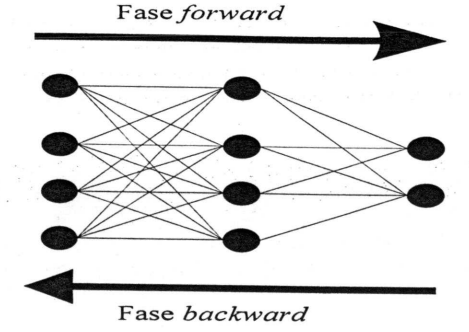
\includegraphics[scale=0.5]{imagens/etapas_MLP.png}
	\end{center}
	\legend{Fonte: \citeonline[p.60]{braga2000redes}}
\end{figure}

\section{Mapas Auto Organizáveis de Kohonen}
\citeonline{kohonen2013essentials} define SOM como uma técnica de análise de dados não supervisionado, realizada por meio do treinamento de um \emph{grid} de neurônios. A anélise de sinais chamada \emph{"Vector Quantization"}, introduzido por \citeonline{forgy1965cluster} para forma vetorial, e por \citeonline{lloyd1982least} para dados escalares, foi a base para a criação desta técnica. 

O SOM realiza uma projeção não linear do espaço de dados de entrada, em $\emph{R}^D$, para o espaço de dados do arranjo, em $\emph{R}^P$, executando uma redução dimensional quando \emph{P} < \emph{D}. Como o arranjo é normalmente unidimensional ou bidimensional, então \emph{P} = 1 ou \emph{P} = 2. Ao realizar esta projeção não linear, o algoritmo tenta preservar ao máximo a topologia do espaço original, ou seja, procura fazer com que neurônios de vizinhos no arranjo apresentem vetores de pesos que retratem as relações de vizinhança entre os dados. Para tanto, os neurônios competem para representar cada dado, e o neurônio vencedor tem seu vetor de pesos ajustados na direção do dado. Esta redução da dimensionalidade com preservação topologica permite ampliar a capacidade de análise de agrupamentos dos dados pertecentes a espaços de elevada dimensão.\cite[p.37]{zuchini2003aplicaccoes}

\subsection{Definição Matemática do SOM}

\citeonline{kohonen2007kohonen} faz a seguinte definição matématica para o SOM:

Os primeiros itens de dados que são vetores euclidianos de n-dimensões devem ser considerados 
$$x(t) = [\xi_1(t),\xi_2(t)\ldots, \xi_\emph{n}(t)]. $$
Para uma determinada sequência, $t$ representa o índice de cada item. Onde o \emph{i}-ésimo modelo será $m_\emph{i}(t) = [\mu_{\emph{i}1}(t),\mu_{\emph{i}2}(t),\ldots,\mu_{in}(t)]$, desta vez $t$ representa o indice na sequência em que são gerados os modelos. Essa sequência é um processo de suavização no qual o novo valor $m_\emph{i}(t + 1)$ é computado iterativamente a contar do valor antigo $m_\emph{i}(t)$ e o novo item $x(t)$, determinado por $$m_\emph{i}(t + 1) = m_\emph{i}(t) + \alpha(t)h_{\emph{ci}(t)}[x(t) - m_\emph{i}(t)].$$
Onde $\alpha(t)$ é um fator escalar que define o tamanho da correção, esse valor decresce a cada época, isto é, a cada novo indice $t$. O indice $i$ se refere ao modelo em processamento, enquanto o indice $c$ refere-se ao modelo com a menor distanfica de $x(t)$ no espaço euclidiano. O fator $h_{ci}(t)$ é a função de vizinhança. É igual a 1 quando $i = c$ e o valor decresce a medida que a distância entre os modelos $m_i$ e $m_\emph{c}$ aumenta no grid. Além diso, a cada época a largura espacial do kernel no grid diminui. As funções que determinam a convergência, devem ser escolhidas com muita cautela.

Ainda segundo \citeonline{kohonen2007kohonen} embora o algoritmo iterativo tenha sido usado com êxito em  incontáveis aplicações, foi expôsto que o esquema \emph{Batch Map} produz resultados essencialmente semelhantes, mas com maior velocidade. A idéia básica é que para cada no $j$ no grid, a média $\bar{x}(t)$ de todos os itens de entrada $x(t)$ é formada e tem $m_j$ como modelo mais próximo. Após isso, os novos modelos são computados como $$m_i = \sum_jn_jh_{ji}\bar{x}_j/\sum_j n_j h_{ji}$$ onde $n_j$ é o número de itens de entrada mapeados para o nó $j$, e o índice $j$ é executado  para toda vizinhançado do nó $i$. Esse esquema é iterado alguma vezes para o $m_i$ atualizado, sempre utilizando o mesmo lote de itens de dados de entrada para determinar o novo $\bar{x}_j$.
%devo colocar o algortimo convencional?
\subsection{Aprendizagem}

O algoritmo básico de trinamento do SOM consiste em três fases. Na primeira fase, competitiva, os neurônios da camada de saída competem entre si, segundo algum critério, geralmente a distância Euclideana, para encontrar um único vencedor, também chamado de BMU (\emph{Best Match Unit}). Na segunda fase, cooperativa, é definida a vizinhança deste neurônio. Na ultima fase, adaptativa, os vetores de peso do neurônio vencedor e de sua vizinhança são ajustados.\cite[p.34]{da2004mapas}

Conforme \citeonline{sassi2006arquitetura} um mapa entre um espaço discreto de $M$ neurônios e um espaço N-dimensional contínuo de vetores $x$ de entrada, é implementada em uma rede do tipo o-vencedor-fica-com-tudo. Neste caso um neurônio vencedor pode representar mais de um vetor $x$. Portanto, este neurônio será o representante de um grupo de padrões $x$ que o fazem ser vencedor. Esse neurônio é adaptado (\emph{winner-takes-all}). O vetor de pesos associado a ele é atualizado de forma a representar ainda mais o dado apresentado, aumentando a probabilidde de que este mesmo neurônio volte a vencer em uma próxima apresentação de dado semelhante, ou do mesmo dado.

Segundo \citeonline{zuchini2003aplicaccoes} e \citeonline{sassi2006arquitetura} a idéia fundamental na fase cooperativa e adaptiva, é que neurônios próximos no arranjo representem dados próximos no espaço de dados. A introdução da função de vizinhança faz com que o vetor de pesos não apenas do neurônio vencedor seja atualizado na direção da entrada atual, mas o vetor de pesos dos neurônios que fazem parte de sua vizinhança. \citeonline{sassi2006arquitetura} faz a seguinte analogia, todos o vetores de pesos dos neurônios da rede SOM estariam ligados por elásticos, onde os elásticos de maior intesidade estariam unindo os vetores mais proximos, e conforme a distância entre esses vetores aumenta a intensidade dos elásticos diminui. Quando o vetor peso de um determinado neurônio vencedor fosse alterado, ele arrastaria consigo os demais vetores que estão ligados a ele, e mais intensamente aqueles mais próximos.
\section{K-means}
Conforme \citeonline{lopes2004mineraccao} \emph{clustering} tem sido empregado em um número de aplicações baseadas em texto tais como Recuperação de informação e Categorização de textos. O \emph{clustering} é o agrupamento de representaçãoes similares de documentos em  separações onde os documenos pertencentes a mesma partição possuem uma similaridade maior entre eles do que a qualquer outro documento em qualquer outra partição.

O algoritmo K-means, criado por MacQueen em 1967 é o algoritmo de \emph{clustering} mais conhecido e utilizado já que é de aplicação muito simples e eficaz. Segue um procedimento simples de classificação de um conjunto de objetos em um determinado número K de \emph{clusters}, onde o K é determinado a priori.\cite{cambronero2006algoritmos}

Ainda segundo \citeonline{cambronero2006algoritmos} o algoritmo recebe tal nome por causa do seu funcionamento, já que o mesmo cria \emph{clusters} a partir da média (ou média ponderada) de seus pontos, e assim estabelece o centróide. Este tipo de representação tem a vantagem de possuir um significado gráfico e estátistico imediato. Cada agrupamento é caracterizado pelo seu centróide, que por sua vez está no centro e na média de todos os elementos que compõem o \emph{cluster}.

Dado um número fixo de k, o \emph{clustering} K-means cria um conjunto de k \emph{clusters} e distribui o conjunto de documentos dados entre esses \emph{clusters} usando a similaridade entre os vetores-documento e os centróides dos \emph{clusters}, Um centróide é o vetor médio de todos os vetores-documento no respectivo \emph{cluster}. Cada vez que se adiciona um documento em um \emph{cluster}, o centróide daquele \emph{cluster} é recalculado. Note que quase sempre, um centróide não corresponde a um documento. A similaridade entre um documento \emph{d} e um centróide \emph{c} é calculada como o somatório de todos os vetores-documento no \emph{cluster} dividido pelo número de vetores-documento.\cite[p.53]{lopes2004mineraccao}

\section{Visualização de dados}
De acordo com \citeonline{freitas2008extraccao} a aplicação do termo visualização hoje é associada à possibilidade de explorar as informaçãoes subjacentes à representação gráfica. Porém genericamente, visualização é entendida como a "representação grafica de dados ou conceitos" \apudonline{warecolin2001}{freitas2008extraccao}.

Conforme descrito por \citeonline{do2005visualizaccao} o processo de visualização está associado a geração de imagens (mentais ou reais) que possam ser analisadas pelos seres humanos a partir de algo abstrato. O objetivo final é facilitar o entendimento de um assunto determinado, onde o mesmo exigiria maior esforço para ser compreendido. Uma vez que técnicas que facilitam o entendimento de informações a partir de representações visuais de dados são agregados a área de Visualização de Informações, o estudo neste campo apresenta grande utilidade. Na área da Computação, a visualização de informações possue um destaque especial nas áreas de mineração de dados e na engenharia de software, pois auxilia na análise e no entendimento de determinadas estruturas com um maior nivel de abstração.
\subsection{Word cloud}
Conforme \citeonline{sargiani2018identificaccao} nuvens de palavras (\emph{word cloud}) são visualizações gráficas onde as palavras, de acordo com sua relevância dentro do \emph{Corpus} de origem, assumem posição e tamanho defirentes. Cores diferentes também podem ser usadas para auxiliar na diferenciação das palavras, e a própria nuvem de palavras pode ser formatada de acordo com o objetivo de transmissão de conhecimento que se espera.

Como exposto por \citeonline{heimerl2014word} uma popular área de aplicação para \emph{word cloud} é a sumarização de texto. Neste contexto as nuvens são utilizadas para que uma visão geral intuitiva e visualmente atraente seja fornecida. Tal sumarização é proveitosa para aprendizagem sobre o número e tipo de temas presentes no corpo do texto. Essa visão estatística é gerada pelo correlacionamento entre o tamanho da fonte das palavras representadas com a frequência das mesmas. 

Esta técnica foi originada on-line na década de 1990 como nuvens de tags, que foram utilizadas para exibir a popularidade de palavras-chave em bookmarks, consoante \citeonline{harris2011word}.
\chapter{Desenvolvimento}
\section{Obtenção dos Dados}
\section{Pré Processamento}
\section{Análise}
\section{Treinamento SOM e K-Means}
\section{Treinamento MLP}
\chapter{Testes e Análise de Resultados}
\chapter{Conclusão}
% ---
% ----------------------------------------------------------
% ELEMENTOS PÓS-TEXTUAIS
% ----------------------------------------------------------
\postextual
% ----------------------------------------------------------
% ----------------------------------------------------------
% Referências bibliográficas
% ----------------------------------------------------------
\bibliography{Referências}

% ----------------------------------------------------------
% Glossário
% ----------------------------------------------------------
%
% Consulte o manual da classe abntex2 para orientações sobre o glossário.
%
%\glossary

% ----------------------------------------------------------
% Apêndices
% ----------------------------------------------------------

% ---
% Inicia os apêndices
% ---

% Imprime uma página indicando o início dos apêndices
\partapendices

% ----------------------------------------------------------

%---------------------------------------------------------------------
% INDICE REMISSIVO
%---------------------------------------------------------------------
\phantompart
\printindex
%---------------------------------------------------------------------

\end{document}
